\section{Descrizione del rilievo topografico e nozioni teoriche}

\subsection{Il rilievo topografico}
Con rilievo topografico si intende il processo con cui avviene la misurazione ed il seguente inquadramento geografico di una porzione di terreno.\\
Per fare ciò, vengono determinate le posizioni di un certo numero di punti dell'area d'interesse; questo è dovuto all'impossibilità di considerare tutti i punti dell'oggetto. Ne deriva la necessarietà di distinguere i punti che vengono acquisiti, in base al loro grado di importanza e di precisione (di inquadramento e di dettaglio).\\
In questo rilievo, data l'estensione del rilievo e dato l'utilizzo di un unico strumento di misura, i punti acquisiti non vengono distinti.
\subsection{Poligonazioni}
La poligonazione è un metodo con cui, mediante una serie di segmenti, si collegano dei punti sul terreno (detti vertici della poligonale), al fine di svolgere il rilievo topografico della relativa area.\\
Una poligonale può essere di diverse tipologie:
\begin{itemize}
    \item aperta: i due estremi sono distinti;
    \item chiusa: i due estremi sono coincidenti. La compensazione degli errori risulta più efficace;
    \item orientata: i punti sono riferiti ad un sistema di riferimento noto;
    \item locale: i punti non sono riferiti ad un sistema di riferimento noto, bensì scelto dall'operatore.
\end{itemize}
La delimitazione di una poligonale può avvenire conoscendo tutti i parametri angolari (per gli angoli al vertice) e tutti quelli lineari dei segmenti che la compongono.\\
L'utilizzo della poligonale, oltre ad avere vantaggio di semplicità, porta con se uno svantaggio importante: essendo i vertici dipendenti dalle misure angolari e lineari dei punti precedenti, la propagazione degli errori risulta rapida.\\
Fortunatamente, soprattutto con le poligonali chiuse, è possibile svolgere la compensazione degli errori, rendendo quindi il risultato finale più prossimo a quello reale. Per le poligonali chiuse sono presenti due elementi sovrabbondanti, che verranno proprio utilizzati per controllare e compensare il risultato finale.\\
Gli angoli della figura poligonale possono essere di due tipologie: interni e azimutali. Gli angoli interni sono gli angoli compresi tra i due segmenti della figura piana. Gli angoli azimutali indicano l'ampiezza angolare tra il segmento preso in considerazione e l'asse di orientamento precedentemente scelto.\\
Nel caso di questa relazione, la poligonale risulta essere chiusa e locale.
\begin{figure}[H]
    \centering
    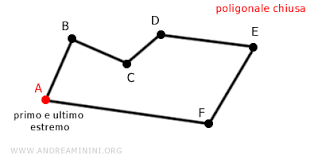
\includegraphics[width=0.5 \textwidth]{immagini/poligonale_chiusa.png}
    \caption{Esempio di una stazione poligonale chiusa.}
    \label{fig:poligonale_chiusa}
\end{figure}

\subsection{Stazione totale}
La stazione totale è uno strumento digitale, che permette di eseguire misurazioni angolari e lineari, in modo da effettuare rilievi topografici.\\
La stazione totale è costituita essenzialmente da tre elementi:
\begin{itemize}
    \item il sistema base-basetta: è solidale al treppiede, supporta ed inclina tutto lo strumento;
    \item l'alidada: permette l'inclinazione verticale dello strumento;
    \item il cannocchiale: è solidale all'alidada, è permette di mirare all'obiettivo di misura.
\end{itemize}
\begin{figure}[H]
    \centering
    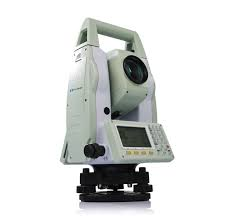
\includegraphics[width=0.4 \textwidth]{immagini/stazione_totale.jpg}
    \caption{Esempio di una stazione totale, comprendente del sistema base-basetta, alidada e cannocchiale.}
    \label{fig:stazione_totale}
\end{figure}
La stazione totale possiede tre assi differenti: uno sul quale ruota l'alidada, uno sul quale ruota il cannocchiale ed uno solidale con i primi due.\\
Gli angoli misurabili dalla stazione totale possono essere sia zenitali (rispetto all verticale) e sia azimutali (rispetto all'orizzontale): tali angoli sono misurabili grazie ai due cerchi, uno verticale ed uno orizzontale.\\
Al fine di effettuare misurazioni il più possibili corrette e ripetibili, è necessario porre questo strumento di misura coincidente alla verticale. Per fare ciò si utilizzano tre diversi sistemi di livellazione, ed ognuno con una diversa precisione. In ordine crescente di precisione:
\begin{itemize}
    \item livella sferica sulla basetta, la cui precisione è mediamente di 4'/2mm-8'/2mm;
    \item livella torica sull'alidada, la cui sensibilità è solitamente di 10''/mm-20''/mm;
    \item livella elettronica interna al circuito elettronico della stazione totale.
\end{itemize}
Al fine di ricavare la misura angolare e lineare di una determinata posizione, è necessario che la stazione totale miri ad un preciso obiettivo, posto precisamente nel punto di interesse. Tale obiettivo è generalmente rappresentato da un prisma topografico, posto al di sopra di una palina.\\
Essendo stato utilizzato lo stesso strumento di misura, è lecito considerare la distribuzione degli errori (angolari e lineari) omogenei per tutta la poligonale. Nel caso degli angoli, la somma degli errori prende il nome di ``errore di chiusura angolare"; mentre, la somma degli errori lineari dei segmenti prende il nome di ``errore di chiusura lineare''.\\

